% !Mode:: "TeX:UTF-8"
\thispagestyle{empty}  
\chapter{2D Laser Localization and Mapping}  
\thispagestyle{empty}  
\label{cpt:2d-mapping}  
In the previous chapter, we introduced the basic principles of laser measurement, as well as the nearest neighbor and fitting methods for point clouds. These serve as the foundation for most laser point cloud registration methods. However, people often treat 2D and 3D laser processing scenarios differently. Overall, 2D laser registration is easier and more suitable for introducing image-like processing methods. This chapter will introduce the relatively simpler 2D laser SLAM, while the next chapter will cover 3D laser SLAM systems. Readers can compare the differences between the two systems from theoretical and methodological perspectives.  

\includepdf[width=\textwidth]{art/ch6.pdf}

\section{Basic Principles of 2D Laser SLAM}

\begin{figure}[!htp]  
	\centering  
	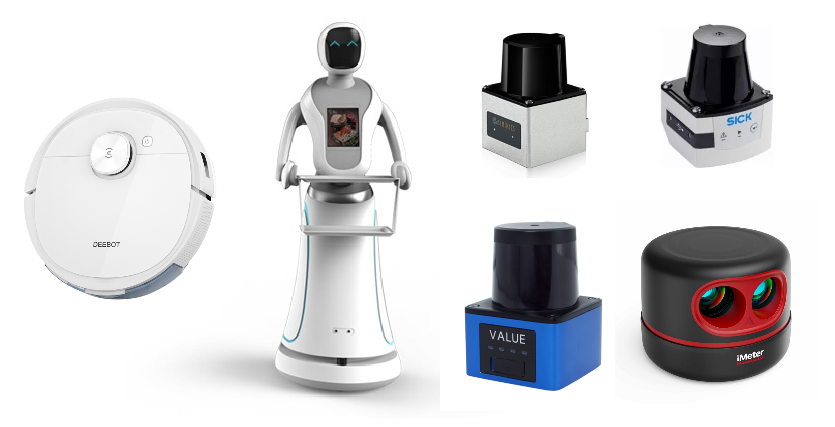
\includegraphics[width=0.8\textwidth]{resources/2d-lidar-mapping/2d-robots.pdf}  
	\caption{Robots using 2D laser SLAM and their corresponding lidars. Cleaning robots typically mount lidars on top, while service robots have built-in lidars after slotting at the base.}  
	\label{fig:2d-robots}  
\end{figure}  

All real-world sensors naturally operate in three-dimensional space, inherently without any distinction of dimensionality. However, most wheeled robots move only on a fixed plane, unlike aircraft that freely change their posture. Cleaning robots operate on horizontal ground, while wall-climbing robots work on vertical planes. Some robots, such as hotel food delivery robots, may have a certain height in their main body, but the part primarily responsible for movement—and thus the main focus of SLAM algorithms—is two-dimensional, as shown in Figure~\ref{fig:2d-robots}.  

Compared to point clouds in three-dimensional space, 2D SLAM can be viewed as a laser SLAM algorithm operating from a top-down perspective. From this viewpoint, laser scan data and map data can be simplified into two-dimensional forms. They closely resemble images, and the map itself can even be stored as an image. Some image feature extraction and matching algorithms can also be applied to 2D SLAM. 2D SLAM is crucial for applications like cleaning robots and AGVs (Automated Guided Vehicles) and was once the dominant focus of SLAM technology \cite{Thrun2005} (it remains the most widely deployed field today). Historically, it has given rise to many well-known methods, such as FastSLAM \cite{Montemerlo2002}, GMapping \cite{Grisetti2007a}, and others.  

However, due to the assumption of planar motion, when the robot body or the environment contains significant three-dimensional objects, some fundamentally unsolvable problems arise at the system level. For example, most 2D SLAM solutions assume obstacles are at the same height as the laser sensor. If the environment contains obstacles at other heights or objects whose shapes vary noticeably with height (e.g., a tabletop and its legs are clearly different), 2D maps struggle to represent such objects, and the robot may collide with them. Another example is when the robot moves on an inclined slope, where the scanned object distances differ geometrically from the actual distances. These scenarios violate the 2D motion assumption and are inherent limitations of the system, making them difficult to resolve within the framework of 2D SLAM. The 3D point cloud SLAM introduced in the next chapter can effectively address these shortcomings caused by 2D assumptions.  

On the other hand, early 2D SLAM systems often treated the map as a single 2D image, an approach that was simplistic and not well-suited for handling loop closures. This chapter will introduce 2D SLAM from a more modern perspective, adopting a framework similar to that of 3D laser SLAM. The content arrangement will also emphasize the similarities between the two.  

\begin{figure}[!htp]  
	\centering  
	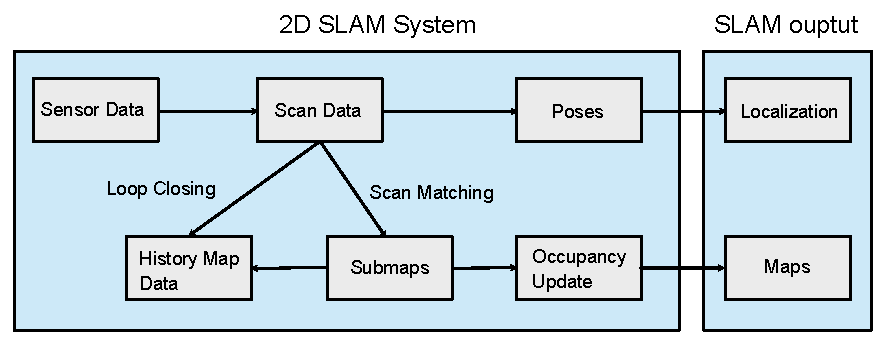
\includegraphics[width=0.8\textwidth]{resources/2d-lidar-mapping/2d-slam-pipeline.pdf}  
	\caption{The basic pipeline of submap-based 2D SLAM.}  
	\label{fig:2d-slam-pipeline}  
\end{figure}  

Figure~\ref{fig:2d-slam-pipeline}~illustrates a typical 2D SLAM framework. Here is a brief overview of its workflow:  

\begin{enumerate}  
	\item First, the 2D laser sensor outputs range measurements at a fixed frequency. Each full cycle of data is called a \textbf{scan} \footnote{Hereafter, the term "scan" will refer to the laser scan data within one cycle. Since terms like "scan-to-scan" are already widely used in the industry, we will not deliberately translate "scan."}.  
	\item To estimate the robot's pose for this scan, we need to \textbf{match} (or \textbf{register}) it against something. This process is called \textbf{scan matching}. We can match the scan either against the previous scan or against the map, so scan matching can be further divided into \textit{scan-to-scan} and \textit{scan-to-map} modes. The principles are largely the same, and they can be used flexibly in practice. In this chapter, we will implement common 2D scan matching algorithms, such as point-to-point and point-to-line methods.  
	\item After estimating the pose of this scan, we integrate it into the map. Of course, a scan is essentially a point cloud, so the simplest approach is to place all scans into the map in chronological order. However, this may suffer from cumulative errors or moving objects. Modern SLAM solutions often adopt a more flexible \textbf{submap} approach, grouping nearby laser scans into a submap and then stitching the submaps together \cite{Hess2016}. In the submap model, each submap is internally fixed and does not require repeated computation. At the same time, submaps have their own independent coordinate systems, and the poses between them can be adjusted and optimized. Thus, when handling loop closures, submaps can be treated as basic units. Early SLAM solutions often relied on a single global map \cite{Grisetti2007a}. Submaps represent an intermediate management approach between single frames and a full map, making loop closure detection and map updates more convenient. This chapter will also adopt the submap model for map construction.  
	\item Finally, how should the scanned map be stored and updated? Many robot maps need to distinguish between \textbf{obstacles} and \textbf{navigable areas}. To represent these concepts, we will use an \textbf{occupancy grid map} for map management \cite{Thrun2003a, MeyerDelius2012}. Occupancy grid maps can effectively filter out the impact of moving objects, resulting in cleaner maps.  
\end{enumerate}  

In this chapter, we will work with readers to implement the mainstream 2D SLAM algorithms discussed above. We will implement several key scan matching algorithms, build them into local submaps, and then use loop closure corrections to construct a complete occupancy grid map. Among the algorithms mentioned here, scan matching is the core of many subsequent processes. We can use traditional methods like the Iterative Closest Point (ICP) algorithm for scan matching or leverage the characteristics of 2D to implement image-based methods such as Gaussian likelihood fields.

\section{Scan Matching Algorithms}  
\subsection{Point-to-Point Scan Matching}  

Let us begin by introducing the scan matching methods in 2D SLAM. A single 2D scan is represented by a set of angle-distance pairs, denoted as $(\rho, r)_i$, where $\rho$ is the angle relative to the robot's own frame, $r$ is the measured distance, and $i = 0, \ldots N$ indicates multiple measurement points. The value of $N$ depends on the angular resolution of the laser sensor. In implementation, these data points are often stored in an array. These measurements are in polar coordinates and can be naturally converted to Cartesian coordinates, expressed as $(x,y)_i$.  

\subsubsection{Visualizing 2D Lidar Data Using OpenCV}  

Starting from this chapter, we will use real-world data collected from actual robots to verify whether our algorithms perform satisfactorily in real-world scenarios. This section and subsequent chapters will require some ROS bag files. Due to their large size, readers are advised to download the necessary datasets from the code repository associated with this book. If storage space is limited, you may choose to download only representative datasets for each chapter. The program in this section requires the data package located in the `2dmapping/` directory, while other chapters will use datasets from their respective directories.  

To facilitate testing different algorithms across various datasets, we have implemented an abstract interface for ROS bag processing. Readers only need to define callback functions for different message types. For example, in the demo code shown here, we need to read 2D scan messages from the bag file and pass them to a visualization program for rendering. In other chapters, these data may be fed into matching algorithms for registration. We leverage C++ lambda functions to achieve this flexible invocation:  

\begin{lstlisting}[language=c++,caption=src/ch6/test\_2dlidar\_io.cc]  
sad::RosbagIO rosbag_io(FLAGS_bag_path);  
rosbag_io  
.AddScan2DHandle("/pavo_scan_bottom",  
	[](Scan2d::Ptr scan) {  
		cv::Mat image;  
		sad::Visualize2DScan(scan, SE2(), image, Vec3b(255, 0, 0));  
		cv::imshow("scan", image);  
		cv::waitKey(20);  
		return true;  
	})  
.Go();  

void Visualize2DScan(Scan2d::Ptr scan, const SE2& pose, cv::Mat& image, const Vec3b& color, int image_size, float resolution, const SE2& pose_submap) {  
	if (image.data == nullptr) {  
		image = cv::Mat(image_size, image_size, CV_8UC3, cv::Vec3b(255, 255, 255));  
	}  
	
	for (size_t i = 0; i < scan->ranges.size(); ++i) {  
		if (scan->ranges[i] < scan->range_min || scan->ranges[i] > scan->range_max) {  
			continue;  
		}  
		
		double real_angle = scan->angle_min + i * scan->angle_increment;  
		double x = scan->ranges[i] * std::cos(real_angle);  
		double y = scan->ranges[i] * std::sin(real_angle);  
		
		if (real_angle < scan->angle_min + 30 * M_PI / 180.0 || real_angle > scan->angle_max - 30 * M_PI / 180.0) {  
			continue;  
		}  
		
		Vec2d psubmap = pose_submap.inverse() * (pose * Vec2d(x, y));  
		
		int image_x = int(psubmap[0] * resolution + image_size / 2);  
		int image_y = int(psubmap[1] * resolution + image_size / 2);  
		if (image_x >= 0 && image_x < image.cols && image_y >= 0 && image_y < image.rows) {  
			image.at<cv::Vec3b>(image_y, image_x) = cv::Vec3b(color[0], color[1], color[2]);  
		}  
	}  
	
	// Draw the robot's position  
	Vec2d pose_in_image =  
	pose_submap.inverse() * (pose.translation()) * double(resolution) + Vec2d(image_size / 2, image_size / 2);  
	cv::circle(image, cv::Point2f(pose_in_image[0], pose_in_image[1]), 5, cv::Scalar(color[0], color[1], color[2]), 2);  
}  
\end{lstlisting}  

As shown, this program uses the `sad::RosbagIO` class to read the `pavo_scan_bottom` messages from the bag file and passes them to a visualization function. The visualization function converts the lidar's range and angle measurements into Cartesian coordinates and renders them onto an image at a specified resolution. If the robot's pose is provided, the visualization can also display the scan data in motion. Here, we demonstrate the scan data in the robot's body frame by setting the input pose to the origin.

Now, please compile the `test_2dlidar_io` program and run the following command to view the laser scan data in the given bag file:

\begin{lstlisting}[language=sh, caption=Terminal command]
	/bin/test_2dlidar_io --bag_path ./dataset/sad/2dmapping/floor1.bag
\end{lstlisting}

Readers should see laser scan data similar to Figure~\ref{fig:2dscan}. Since the actual robot was moving, you should also observe structures from different locations in the scene. With good spatial imagination, one should be able to infer the robot's movement direction and surrounding environment.

\begin{figure}[!htp]
	\centering
	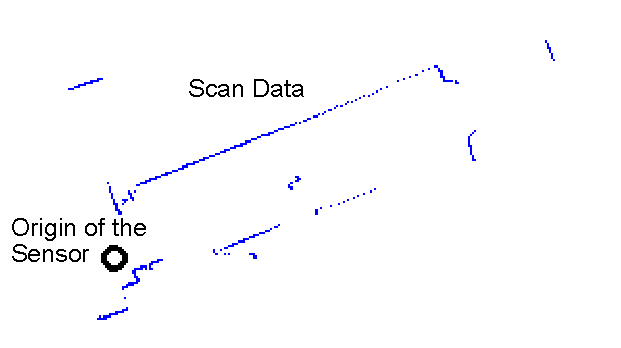
\includegraphics[width=0.5\textwidth]{resources/2d-lidar-mapping/2dscan}
	\caption{Example of single 2D scan data}
	\label{fig:2dscan}
\end{figure}

In scan data like Figure~\ref{fig:2dscan}, we call the actual laser hit points \textbf{end points}. End points have two physical meanings:
1. The end point itself represents an actual existing obstacle;
2. Along the line connecting the sensor to the end point, no other obstacles exist.

Note that the second meaning requires calculating the line from the sensor to the end point (the sensor doesn't measure this line - it only measures the end point, so we need to compute this line ourselves). If we want to calculate which grid cells this line passes through, it involves \textbf{ray casting algorithm} \cite{Ray1999} and \textbf{rasterization algorithm} \cite{Pineda1988}. We'll mention these again later in grid map construction and provide a simple implementation. However, in scan matching algorithms, we focus more on the first meaning and often ignore the second.

Under this premise, a single scan can be viewed as a simple 2D point set.

Now let us derive the mathematical model for scan matching algorithms. From the perspective of state estimation, 2D laser scan data can be denoted as observation data $\bm{z}$. It is obtained when the robot at pose $\bm{x}$ observes a certain map $\bm{m}$. Thus, the observation model can be simply expressed as:
\begin{equation}\label{key}
	\bm{z} = \bm{h} (\bm{x}, \bm{m}) + \bm{w},
\end{equation}
where $\bm{w}$ is the noise term. Our goal is to estimate $\bm{x}$ based on the observed $\bm{z}$ and $\bm{m}$. According to Bayesian estimation theory, $\bm{x}$ can be obtained through \textbf{Maximum a Posteriori} (MAP) or \textbf{Maximum Likelihood Estimation} (MLE):
\begin{equation}\label{key}
	\bm{x}_{\mathrm{MLE}} = \arg \max p(\bm{x}|\bm{z}, \bm{m}) = \arg \max p(\bm{z}|\bm{x}, \bm{m}).
\end{equation}

If we only consider the scan-to-scan problem, $\bm{m}$ can simply be written as the previous scan data. The key then becomes how to define the detailed form of the observation equation, i.e., how to compute the residual term for each observation. Here we present several typical solutions: point-to-point scan matching (ICP) \cite{Arun1987}, point-to-line scan matching (PL-ICP \cite{Censi2008} or ICL \cite{Alshawa2007}), and the Gaussian likelihood field method (or CSM \cite{Olson2009}). In 3D matching algorithms, we will further introduce other methods such as point-to-plane \cite{Park2003,Low2004} and NDT \cite{Biber2003,Magnusson2009,Rapp2015}. Since 2D scan matching does not involve surface elements, we will only discuss point-to-point and point-to-line algorithms here.

The specific definition of the observation equation involves several issues:
\begin{enumerate}
	\item How to select the points to be matched. In principle, all scanned points should participate in matching, but for efficiency considerations, \textbf{sampling} can be applied. There are many sampling methods, from uniform or random sampling to normal- or feature-based sampling, all of which can be used in practice.
	\item How to determine which specific map point corresponds to a scan point $(x,y)_i$. This is also known as the \textbf{data association} problem. This problem is typically solved using the nearest neighbor method introduced in the previous section, i.e., assuming that under the current estimated pose, the closest map point to the observed point is the matching point. In field-based methods, grid cells or fields in the map can also be used as matching points.
	\item After determining the scan point $(x,y)_i$ and its corresponding map point $\bm{m}_i$, how to compute the residual. This involves the modeling of residuals. The complete laser scan noise model (beam model) is complex with many parameters \cite{Cabaleiro2015}, and as a state estimation model, it is not smooth enough. In practice, we usually simplify it, and in the simplest case, we can directly model it as a 2D Gaussian distribution, i.e., $\bm{w} \sim \mathcal{N}(\bm{0}, \boldsymbol{\Sigma})$.
\end{enumerate}

As can be seen, a scan matching algorithm involves many choices at different stages, and there are numerous variants of basic methods in both industry and academia. We will introduce the origins of these variants starting from basic methods, but we will not attempt to cover all scan matching algorithms. To maintain consistency, we will use the same mathematical notation to describe the problems and provide code implementations for each algorithm.

First, let us look at the simplest point-to-point matching problem, also known as the Iterative Closest Point (ICP) algorithm \cite{Besl1992}. The ICP algorithm divides the scan matching problem into two steps: \textbf{data association} and \textbf{pose estimation}, and alternates between these two steps until convergence. In fact, regardless of how data association and pose estimation are specifically solved, as long as the algorithm involves alternating between these two steps, we can refer to it as an \textbf{ICP-like} algorithm \cite{Koide2020,segal2009generalized,Zhang2021a}. When the matching relationship is known, ICP can be solved in closed form, but this approach discards the possibility of further filtering outliers and makes point-to-point and point-to-plane methods appear different (note that from an optimization perspective, they are unified). For consistency, we will describe the problem in terms of residuals and optimization.

The pose of a 2D laser is described by translation and rotation angles\footnote{In the program, we use the SE2 interface, which is essentially the same as the SE3 interface. We can use the same notation for SE3 and SE2, such as matrix multiplication. In some literature, 2D poses are also referred to as \textbf{three-degree-of-freedom} poses.}, and can be simply written as:
\begin{equation}\label{key}
	\bm{x} = [x, y, \theta]^\top.
\end{equation}

Here, $\bm{x}$ describes a transformation from the robot's coordinate frame $B$ to the world frame $W$, denoted as $\bm{x} = \bm{T}_{WB}$ according to the convention of this book. Note that submap frames and their coordinate systems will be introduced later, so it is necessary to clarify the transformation relationship of $\bm{x}$. Suppose a scan point $\bm{p}_i^B$ in the robot's frame has distance and angle $r_i, \rho_i$. Then, based on the current laser pose, it can be transformed to the world frame:
\begin{equation}\label{key}
	\bm{p}^W_i = [x+r_i \cos (\rho_i + \theta), y+r_i \sin(\rho_i + \theta)]^\top.
\end{equation}
In 3D space, this can be written as:
\begin{equation}\label{key}
	\bm{p}^W_i = \bm{T}_{WB} \bm{p}^B_i.
\end{equation}

In the program, since the SE3 and SE2 interfaces are consistent, we do not deliberately distinguish between 3D and 2D poses in mathematical notation.

Assuming we find a nearest neighbor $\bm{q}_i^W$ near $\bm{p}_i^W$, we can easily construct the residual between $\bm{p}_i^W$ and $\bm{q}_i^W$:
\begin{equation}\label{key}
	\bm{e}_i = \bm{p}_i^W - \bm{q}_i^W,
\end{equation}

This residual describes the Euclidean geometric distance between two points. Clearly, this error uses world coordinates and is related to the robot's pose at that time. Thus, the robot pose estimation problem can be transformed into a least-squares problem with variables $x, y, \theta$:
\begin{equation}\label{key}
	(x,y,\theta)^* = \arg \min\limits_{\bm{x}} \sum_{i=1}^n \| \bm{e}_i \|_2^2.
\end{equation}
This least-squares problem can be solved by many existing solvers.

To solve the least-squares problem, we should provide the derivatives of $\bm{e}$ with respect to each state variable. The obvious advantage of 2D poses is that we no longer need to use manifold notation and can directly use the decomposed $x, y, \theta$\footnote{Of course, it is possible to unify them using manifold notation, but it is unnecessary.}. Based on the above definitions, we can easily obtain:
\begin{subequations}\label{key}
	\begin{align}
		\frac{\partial{\bm{e}_i}}{\partial x} &= [1, 0]^\top, \\
		\frac{\partial{\bm{e}_i}}{\partial y} &= [0, 1]^\top, \\
		\frac{\partial{\bm{e}_i}}{\partial \theta} &= [-r_i \sin (\rho_i + \theta), r_i \cos (\rho_i+\theta)]^\top.
	\end{align}
\end{subequations}

We can organize this into matrix form:
\begin{equation}\label{eq:dpw-dx}
	\frac{\partial \bm{e}_i}{\partial \bm{x}} = \begin{bmatrix}
		1 & 0\\
		0 & 1\\
		-r_i \sin (\rho_i + \theta) & r_i \cos (\rho_i+\theta)
	\end{bmatrix} \in \mathbb{R}^{3\times 2}.
\end{equation}

In the subsequent experimental section, we will use this Jacobian matrix to solve the Gauss-Newton method. It is important to note that if the state variables $x, y, \theta$ change, $\bm{q}_i$ will also change, altering the entire problem. If the state variables are initially set far from the optimal solution, $\bm{q}_i$ may be an incorrect point, making ICP-like methods highly dependent on the initial value of optimization. We will continue to discuss this issue later.

\subsection{Implementation of Point-to-Point ICP (Gauss-Newton)}  
Below we implement a 2D point-to-point ICP method by manually coding the Gauss-Newton approach. In each Gauss-Newton iteration, we recompute the nearest neighbors between points and then solve for the pose increment. The key points here are: (1) implementing nearest neighbor search, and (2) implementing Gauss-Newton iteration.  

Since the nearest neighbor data structure from the previous lecture used 3D points rather than 2D points, here we employ PCL's K-d tree for nearest neighbor search with 2D points. Thus, when setting the target point cloud, we need to build a K-d tree for it. Our 2D ICP class interface is as follows:  

\begin{lstlisting}[language=c++,caption=src/ch6/icp\_2d.h]  
	class Icp2d {  
		public:  
		using Point2d = pcl::PointXY;  
		using Cloud2d = pcl::PointCloud<Point2d>;  
		Icp2d() {}  
		
		/// Set the target scan  
		void SetTarget(Scan2d::Ptr target) {  
			target_scan_ = target;  
			BuildTargetKdTree();  
		}  
		
		/// Set the source scan to be aligned  
		void SetSource(Scan2d::Ptr source) { source_scan_ = source; }  
		
		/// Perform alignment using Gauss-Newton method  
		bool AlignGaussNewton(SE2& init_pose);  
		
		private:  
		// Build K-d tree for the target point cloud  
		void BuildTargetKdTree();  
		
		pcl::search::KdTree<Point2d> kdtree_;  
		Cloud2d::Ptr target_cloud_;  // Target cloud in PCL format  
		
		Scan2d::Ptr target_scan_ = nullptr;  
		Scan2d::Ptr source_scan_ = nullptr;  
	};  
\end{lstlisting}  

The `AlignGaussNewton` function implements 2D ICP based on Gauss-Newton iteration:  

\begin{lstlisting}[language=c++, caption=src/ch6/icp\_2d.cc]  
	bool Icp2d::AlignGaussNewton(SE2& init_pose) {  
		int iterations = 10;  
		double cost = 0, lastCost = 0;  
		SE2 current_pose = init_pose;  
		const float max_dis2 = 0.01;      // Maximum squared distance for nearest neighbors  
		const int min_effect_pts = 20;  // Minimum number of effective points  
		
		for (int iter = 0; iter < iterations; ++iter) {  
			Mat3d H = Mat3d::Zero();  
			Vec3d b = Vec3d::Zero();  
			cost = 0;  
			
			int effective_num = 0;  // Number of effective points  
			
			// Traverse source points  
			for (size_t i = 0; i < source_scan_->ranges.size(); ++i) {  
				float r = source_scan_->ranges[i];  
				if (r < source_scan_->range_min || r > source_scan_->range_max) {  
					continue;  
				}  
				
				float angle = source_scan_->angle_min + i * source_scan_->angle_increment;  
				float theta = current_pose.so2().log();  
				Vec2d pw = current_pose * Vec2d(r * std::cos(angle), r * std::sin(angle));  
				Point2d pt;  
				pt.x = pw.x();  
				pt.y = pw.y();  
				
				// Nearest neighbor search  
				std::vector<int> nn_idx;  
				std::vector<float> dis;  
				kdtree_.nearestKSearch(pt, 1, nn_idx, dis);  
				
				if (nn_idx.size() > 0 && dis[0] < max_dis2) {  
					effective_num++;  
					Mat32d J;  
					J << 1, 0, 0, 1, -r * std::sin(angle + theta), r * std::cos(angle + theta);  
					H += J * J.transpose();  
					
					Vec2d e(pt.x - target_cloud_->points[nn_idx[0]].x, pt.y -  
					target_cloud_->points[nn_idx[0]].y);  
					b += -J * e;  
					
					cost += e.dot(e);  
				}  
			}  
			
			if (effective_num < min_effect_pts) {  
				return false;  
			}  
			
			// Solve for dx  
			Vec3d dx = H.ldlt().solve(b);  
			if (isnan(dx[0])) {  
				break;  
			}  
			
			cost /= effective_num;  
			if (iter > 0 && cost >= lastCost) {  
				break;  
			}  
			
			LOG(INFO) << "iter " << iter << " cost = " << cost << ", effect num: " << effective_num;  
			
			current_pose.translation() += dx.head<2>();  
			current_pose.so2() = current_pose.so2() * SO2::exp(dx[2]);  
			lastCost = cost;  
		}  
		
		init_pose = current_pose;  
		LOG(INFO) << "estimated pose: " << current_pose.translation().transpose()  
		<< ", theta: " << current_pose.so2().log();  
		
		return true;  
	}  
\end{lstlisting}  

The Jacobian matrix here corresponds to the theoretical part introduced earlier. We limit the maximum squared distance for nearest neighbors (set to 0.01) and count the number of valid nearest neighbors, then compute their average error. Finally, the `current_pose` obtained from Gauss-Newton iteration is filled into the return result.

We also write a test program to evaluate the results of 2D ICP:

\begin{lstlisting}[language=c++,caption=src/ch6/test\_2d\_icp\_s2s.cc]
	rosbag_io.AddScan2DHandle("/pavo_scan_bottom",
	[&](Scan2d::Ptr scan) {
		current_scan = scan;
		
		if (last_scan == nullptr) {
			last_scan = current_scan;
			return true;
		}
		
		sad::Icp2d icp;
		icp.SetTarget(last_scan);
		icp.SetSource(current_scan);
		
		SE2 pose;
		if (FLAGS_method == "point2point") {
			icp.AlignGaussNewton(pose);
		} else if (fLS::FLAGS_method == "point2plane") {
			icp.AlignGaussNewtonPoint2Plane(pose);
		}
		
		cv::Mat image;
		sad::Visualize2DScan(last_scan, SE2(), image, Vec3b(255, 0, 0));    // target in blue
		sad::Visualize2DScan(current_scan, pose, image, Vec3b(0, 0, 255));  // source in red
		cv::imshow("scan", image);
		cv::waitKey(20);
		
		last_scan = current_scan;
		return true;
	})
	.Go();
\end{lstlisting}

This program registers the current scan data to the previous scan and visualizes the results using OpenCV. The previous frame is displayed in blue, while the current frame is shown in red. After registration, the two scans should align well with each other. Running this program allows real-time observation of the registration effect, as shown in Figure~\ref{fig:2dicp-s2s}. Readers can also monitor metrics such as the objective function value and the number of valid points for each ICP iteration in the terminal. However, due to the robot's motion, there will inevitably be some discrepancies between the two scans. Previously unexplored areas will appear in the current frame, and dynamic objects or motion distortion in the scan data itself may also interfere with the registration results. We can adjust the thresholds in ICP or parameters in the optimization model to mitigate the impact of dynamic objects to some extent.

This test program is also compatible with the point-to-plane ICP interface discussed later. Readers can use different gflags to test it.

\begin{figure}[!htp]
	\centering
	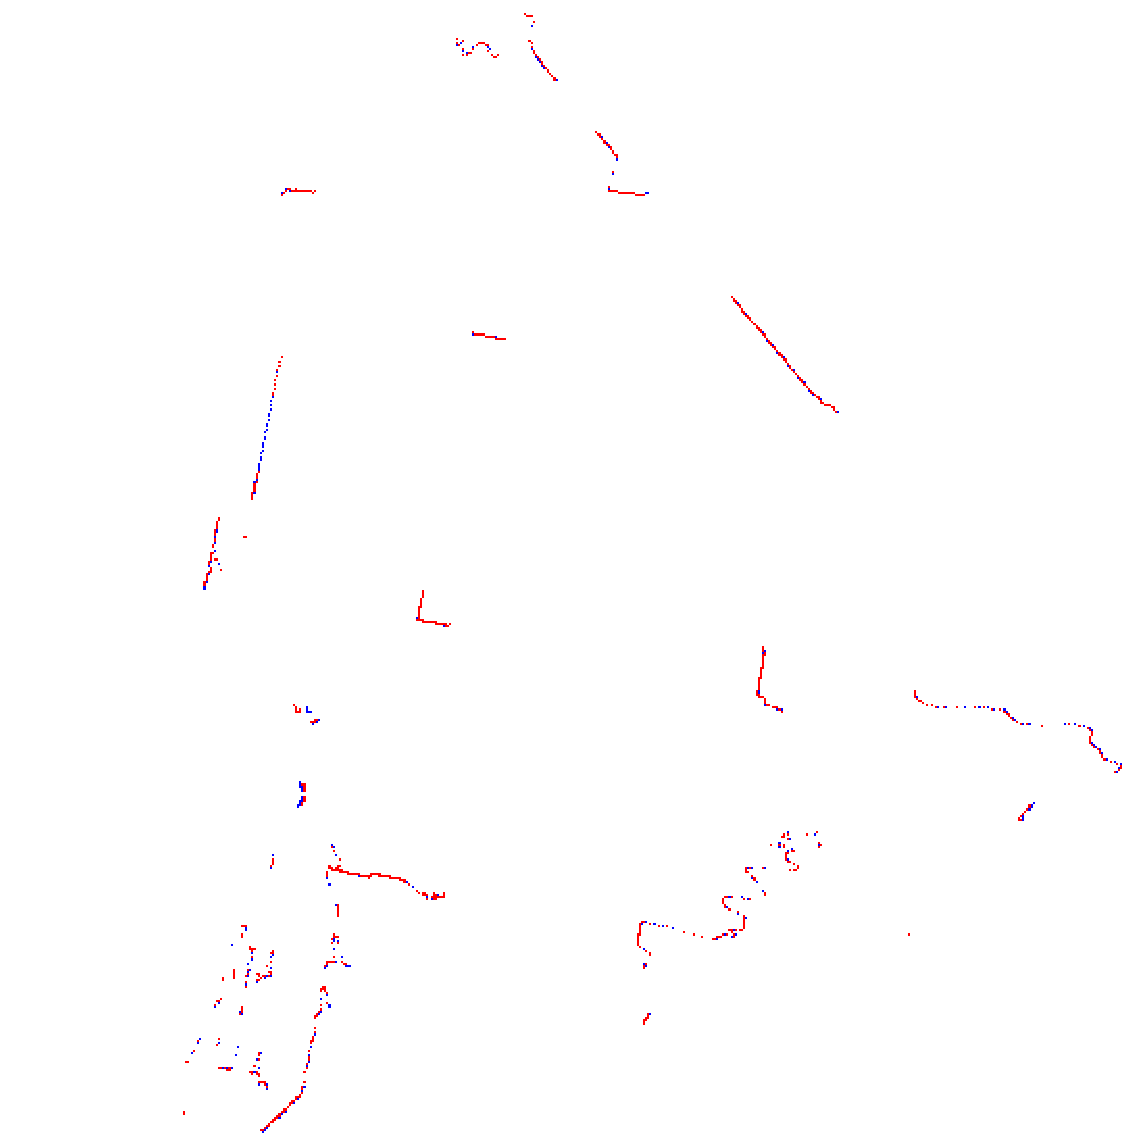
\includegraphics[width=0.4\textwidth]{resources/2d-lidar-mapping/2dicp-s2s}
	\caption{Registration results of point-to-point ICP}
	\label{fig:2dicp-s2s}
\end{figure}

\subsection{Point-to-Line Scan Matching}  
In addition to point-to-point methods, ICP can also utilize other error formulations. The most common alternatives are point-to-line or point-to-plane approaches. Since 2D lidar data doesn't contain planes, we focus on the point-to-line formulation (which can be considered a lower-dimensional version of point-to-plane). The overall workflow of point-to-line ICP remains similar to point-to-point ICP, except that during nearest neighbor search, we need to find multiple neighbors (e.g., k neighbors), fit a line to these points, and then compute the perpendicular distance from the target point to this line. This method is called Point-to-line ICP (PL-ICP) \cite{Censi2008}.

Let these k nearest neighbors be $(\bm{x}_1, \ldots, \bm{x}_k), \forall i \in 1, \ldots k, \bm{x}_i \in \mathbb{R}^2$. In 3D space, the fitted line can be described by a direction vector $\bm{d}$ and origin $\bm{p}$, with fitting methods already introduced in Section~\ref{sec:line-fitting}. While lines in 3D space are more complex, in 2D space they can be simplified to a slope-intercept model. Let the line equation be:
\begin{equation}\label{key}
	a x + by + c = 0,
\end{equation}
where $a,b,c$ are line parameters. The line fitting can then be formulated as a least-squares parameter estimation problem:
\begin{equation}\label{key}
	(a,b,c)^* = \arg \min \sum_{i=1}^N \| a x_i + by_i + c \|_2^2 .
\end{equation}

We simply arrange the point coordinates into a matrix:
\begin{equation}\label{key}
	\bm{A} = \begin{bmatrix}
		x_1 & y_1 & 1 \\
		x_2 & y_2 & 1 \\
		& \ldots &\\
		x_k & y_k & 1
	\end{bmatrix},
\end{equation}
and find the minimum singular vector of $\bm{A}$.

After obtaining the line parameters $(a,b,c)$ from the nearest neighbors, the perpendicular distance from any point $(x,y)$ to this line can be expressed as:
\begin{equation}\label{key}
	d = \frac{ax+by+c}{\sqrt{a^2+b^2}}.
\end{equation}
Since the denominator is a constant that can be ignored, we can directly use the residual:
\begin{equation}\label{key}
	e = ax+by+c,
\end{equation}
as the objective function. The line equation also provides the corresponding Jacobian matrix:
\begin{equation}\label{key}
	\frac{\partial e}{\partial x} = a, \quad \frac{\partial e}{\partial y} = b.
\end{equation}
Thus, the fitted line results can guide the optimization direction. We will see similar results in 3D point-to-plane ICP later.

Now we incorporate the lidar's pose into the above discussion. Let the lidar's position and orientation be $\bm{x} = (x,y, \theta)$. For a lidar point with distance and angle $(r_i, \rho_i)$, we transform it to world coordinates to get $\bm{p}_i^w$. With line parameters $(a_i, b_i, c_i)$ fitted from its nearest neighbors, the Jacobian matrix of its residual $e_i$ with respect to the pose can be expressed using the chain rule:
\begin{equation}\label{key}
	\frac{\partial e_i}{\partial \bm{x}} = \frac{\partial e_i}{\partial \bm{p}_i^w} \frac{\partial \bm{p}_i^w}{\partial \bm{x}},
\end{equation} 
where the latter term is given in Equation \eqref{eq:dpw-dx}, and the former term is determined by the line parameters. Multiplying them together yields:
\begin{equation}\label{key}
	\frac{\partial e_i}{\partial \bm{x}} = [a_i, b_i, -a_i r_i \sin(\rho_i + \theta) + b_i r_i \cos(\rho_i + \theta)]^\top.
\end{equation}


\subsection{Implementation of Point-to-Line ICP (Gauss-Newton)}
Below we implement the algorithm described in the previous section. Its overall workflow is consistent with point-to-point ICP, and we only need to add an interface to the existing ICP class:

\begin{lstlisting}[language=c++,caption=src/ch6/icp\_2d.cc]
	bool Icp2d::AlignGaussNewtonPoint2Plane(SE2& init_pose) {
		int iterations = 10;
		double cost = 0, lastCost = 0;
		SE2 current_pose = init_pose;
		const float max_dis = 0.3;      // Maximum distance for nearest neighbors
		const int min_effect_pts = 20;  // Minimum number of effective points
		
		for (int iter = 0; iter < iterations; ++iter) {
			Mat3d H = Mat3d::Zero();
			Vec3d b = Vec3d::Zero();
			cost = 0;
			
			int effective_num = 0;  // Number of effective points
			
			// Traverse source points
			for (size_t i = 0; i < source_scan_->ranges.size(); ++i) {
				float r = source_scan_->ranges[i];
				if (r < source_scan_->range_min || r > source_scan_->range_max) {
					continue;
				}
				
				float angle = source_scan_->angle_min + i * source_scan_->angle_increment;
				float theta = current_pose.so2().log();
				Vec2d pw = current_pose * Vec2d(r * std::cos(angle), r * std::sin(angle));
				Point2d pt;
				pt.x = pw.x();
				pt.y = pw.y();
				
				// Find 5 nearest neighbors
				std::vector<int> nn_idx;
				std::vector<float> dis;
				kdtree_.nearestKSearch(pt, 5, nn_idx, dis);
				
				std::vector<Vec2d> effective_pts;  // Effective points
				for (int j = 0; j < nn_idx.size(); ++j) {
					if (dis[j] < max_dis) {
						effective_pts.emplace_back(
						Vec2d(target_cloud_->points[nn_idx[j]].x, target_cloud_->points[nn_idx[j]].y));
					}
				}
				
				if (effective_pts.size() < 3) {
					continue;
				}
				
				// Fit line and assemble J, H and error
				Vec3d line_coeffs;
				if (math::FitLine2D(effective_pts, line_coeffs)) {
					effective_num++;
					Vec3d J;
					J << line_coeffs[0], line_coeffs[1],
					-line_coeffs[0] * r * std::sin(angle + theta) + line_coeffs[1] * r * std::cos(angle + theta);
					H += J * J.transpose();
					
					double e = line_coeffs[0] * pw[0] + line_coeffs[1] * pw[1] + line_coeffs[2];
					b += -J * e;
					
					cost += e * e;
				}
			}
			
			if (effective_num < min_effect_pts) {
				return false;
			}
			
			// solve for dx
			Vec3d dx = H.ldlt().solve(b);
			if (isnan(dx[0])) {
				break;
			}
			
			cost /= effective_num;
			if (iter > 0 && cost >= lastCost) {
				break;
			}
			
			LOG(INFO) << "iter " << iter << " cost = " << cost << ", effect num: " << effective_num;
			
			current_pose.translation() += dx.head<2>();        current_pose.so2() = current_pose.so2() * 
			SO2::exp(dx[2]);
			lastCost = cost;
		}
		
		init_pose = current_pose;
		LOG(INFO) << "estimated pose: " << current_pose.translation().transpose()
		<< ", theta: " << current_pose.so2().log();
		
		return true;
	}
\end{lstlisting}

In the implementation, we search for five nearest neighbors around the target point and use them to fit a local line segment. The 2D line fitting algorithm is provided in common/math\_utils.h:

\begin{lstlisting}[language=c++,caption=src/common/math\_utils.h]
	template <typename S>
	bool FitLine2D(const std::vector<Eigen::Matrix<S, 2, 1>>& data, Eigen::Matrix<S, 3, 1>& coeffs) {
		if (data.size() < 2) {
			return false;
		}
		
		Eigen::MatrixXd A(data.size(), 3);
		for (int i = 0; i < data.size(); ++i) {
			A.row(i).head<2>() = data[i].transpose();
			A.row(i)[2] = 1.0;
		}
		
		Eigen::JacobiSVD svd(A, Eigen::ComputeThinV);
		coeffs = svd.matrixV().col(2);
		return true;
	}
\end{lstlisting}

Note its similarity to the 3D plane fitting algorithm. Finally, the test case from the previous section can be used to examine the registration effect of point-to-line ICP. Since its results are similar to point-to-point ICP, we won't include additional figures here - readers are encouraged to experiment themselves (using the test program from the previous section with --method=point2plane). Generally speaking, point-to-line ICP performs better than point-to-point ICP, though at the cost of greater computational requirements due to the need to compute multiple nearest neighbors.

\subsection{Likelihood Field Method}
\label{sec:likelihood-field}

Point-to-point or point-to-line ICP can be used for both scan-to-scan matching and scan-to-map registration. If we store the map as discrete 2D points, ICP-like methods can be applied to map matching in the same way. However, in 2D SLAM, we typically store the map as an \textbf{occupancy grid map} with a certain resolution. This image-like map has an update mechanism that provides some filtering effect against dynamic objects (which we will implement in the next section). Thus, we can design a registration method that aligns scan data with grid maps in an ICP-like manner. The likelihood field method (also known as Gaussian Likelihood Field) introduced in this section is precisely such an approach for registering scan data with grid maps \cite{Thrun2005}.

In point-to-point ICP, we compute Euclidean distance errors between target points and their nearest neighbors in another point cloud. These errors grow with the squared distance between points and ultimately form the objective function through summation. Intuitively, we can imagine a \textbf{spring} installed between each point and its nearest neighbor. The collective pull of these springs eventually brings the point cloud to the position of minimum energy. However, in ICP methods, we must reinstall these springs during each iteration, which is computationally expensive. 

An alternative approach is to consider that the point cloud generates a \textbf{field} in space rather than installing springs between points. This field attracts nearby point clouds, with its attractive force decaying quadratically with distance. This is essentially the idea behind the likelihood field method. We can define a decaying field around each point in the map. Unlike physical fields, however, the fields in computer programs have defined \textbf{effective ranges} and \textbf{resolutions}. The field can decay quadratically or follow a Gaussian distribution with distance. When a measured point falls near the field, we can use the field's value as the error function for that point.

The likelihood field method can be used to register either two scan datasets or a scan dataset with a map dataset. More commonly, it works in conjunction with grid maps for map matching. To perform registration, we first need to generate this likelihood field. In this section, we generate the likelihood field only for point cloud data. Later, after introducing occupancy grid maps, we can also generate likelihood field maps for grid maps. The likelihood field can be further bound with submaps to achieve simple and fast registration. Here, we "draw" a distance-decaying circle around each point. These circles are fixed and can be precomputed.

\begin{figure}[!htp]
	\centering
	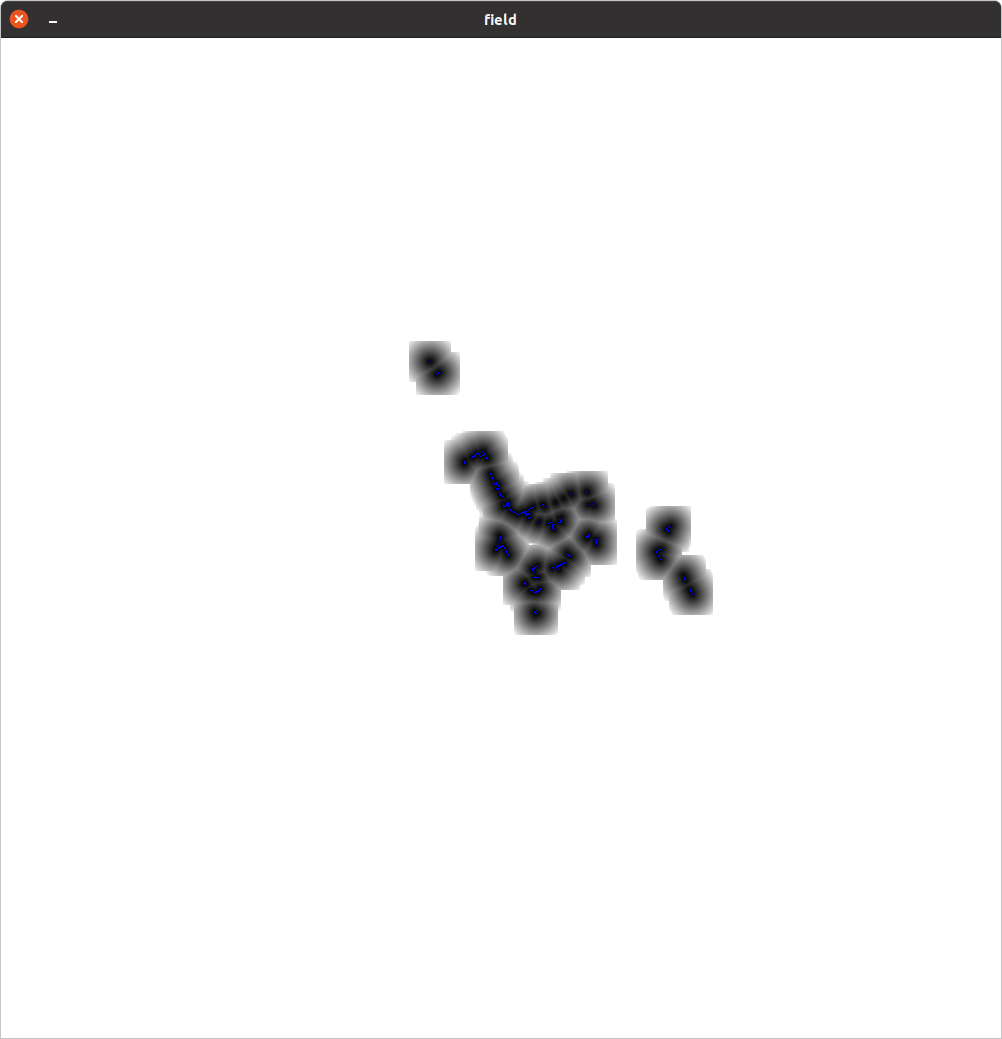
\includegraphics[width=0.5\textwidth]{resources/2d-lidar-mapping/likelihood-field}
	\caption{An example of a likelihood field}
	\label{fig:likelihood-field}
\end{figure}

Figure~\ref{fig:likelihood-field} shows a 2D scan dataset and its corresponding likelihood field. Visually, we can observe that the likelihood field radiates from each scan point and gradually decays with distance. We can customize its range and decay characteristics. The likelihood field essentially describes a distance function between each pixel and its nearest scan point, also referred to as a distance transform map in some applications \cite{Felzenszwalb2012}. With the likelihood field, we no longer need nearest neighbor structures like K-d trees to find the closest point for a given point; instead, we can directly use the field's readings.

Next, we derive the scan matching algorithm based on the likelihood field. The readings from the likelihood field can directly serve as the objective function for registration. Consider a point $\bm{p}^B_i$ transformed by pose $\bm{x}$ to obtain $\bm{p}^W_i$ in the world coordinate frame. Simultaneously, there exists a likelihood field $\pi$ in the world coordinate frame\footnote{Note that the likelihood field doesn't necessarily need to be maintained in the world coordinate frame; later discussions will show it is primarily maintained in submap coordinates.}. The reading of this point in the likelihood field $\pi$ is $\pi(\bm{p}^W_i)$. Thus, $\bm{x}$ can be obtained by solving the optimization problem:
\begin{equation}\label{key}
	\bm{x}^* = \arg \min_{\bm{x}} \sum_{i=1}^{n} \| \pi(\bm{p}_i^W) \|_2^2.
\end{equation}

The Jacobian matrix of the $\pi$ function with respect to pose $\bm{x}$ can be decomposed via the chain rule:
\begin{equation}\label{key}
	\frac{\partial \pi}{\partial \bm{x}} = \frac{\partial \pi}{\partial \bm{p}^W_i} \frac{\partial \bm{p}^W_i}{\partial \bm{x}}.
\end{equation}
The latter term is given in Equation \eqref{eq:dpw-dx}, so we focus on the former term.

Since the likelihood field is stored as an image, $\bm{p}^W_i$ must be sampled at a certain resolution. Let the transformation from $\bm{p}^W_i$ to its image coordinates $\bm{p}^f_i$ be:
\begin{equation}\label{key}
	\bm{p}^f_i = \alpha \bm{p}^W_i + \bm{c},
\end{equation}
where $\alpha$ is the scaling factor and $\bm{c} \in \mathbb{R}^2$ is the offset of the image center. Note that image coordinates typically start from the top-left corner, while object coordinates usually originate from the center, so the offset is typically half the image dimensions. The derivative of function $\pi$ with respect to $\bm{p}^W_i$ is:
\begin{equation}\label{key}
	\frac{\partial \pi}{\partial \bm{p}^W_i} = \frac{\partial \pi}{\partial \bm{p}^f_i} \frac{\partial \bm{p}^f_i}{\partial \bm{p}^W_i}= \alpha [\Delta \pi_x, \Delta \pi_y]^\top,
\end{equation}
where $[\Delta \pi_x, \Delta \pi_y]$ represents the gradient of the likelihood field in the image. Since we define the likelihood function for each point as a smooth function, its gradient is equally reliable. Multiplying these two matrices yields the Jacobian matrix of each residual with respect to the pose:
\begin{equation}\label{key}
	\frac{\partial \pi}{\partial \bm{x}} = [\alpha \Delta \pi_x, \alpha \Delta \pi_y, -\alpha \Delta \pi_x r_i \sin(\rho_i+\theta) + \alpha \Delta \pi_y r_i \cos(\rho_i +\theta)]^\top.
\end{equation}

Using this Jacobian matrix, we can implement registration based on the Gauss-Newton method.

\subsection{Implementation of Likelihood Field Method (Gauss-Newton)}  

When implementing the likelihood field method, we need to generate the corresponding likelihood field when setting the target point cloud. Each point in the likelihood field can use a pre-generated, fixed-size template, which is then "pasted" onto each point of the target point cloud.  

\begin{lstlisting}[language=c++,caption=src/ch6/likelihood\_field.cc]  
	class LikelihoodField {  
		public:  
		/// 2D field template, generated when setting target scan or map  
		struct ModelPoint {  
			ModelPoint(int dx, int dy, float res) : dx_(dx), dy_(dy), residual_(res) {}  
			int dx_ = 0;  
			int dy_ = 0;  
			float residual_ = 0;  
		};  
		
		private:  
		std::vector<ModelPoint> model_;  // 2D template  
	};  
	
	void LikelihoodField::BuildModel() {  
		const int range = 20;  // Template size in pixels  
		for (int x = -range; x <= range; ++x) {  
			for (int y = -range; y <= range; ++y) {  
				model_.emplace_back(x, y, std::sqrt((x * x) + (y * y)));  
			}  
		}  
	}  
	
	void LikelihoodField::SetTargetScan(Scan2d::Ptr scan) {  
		target_ = scan;  
		
		// Generate field function on target points  
		field_ = cv::Mat(1000, 1000, CV_32F, 30.0);  
		
		for (size_t i = 0; i < scan->ranges.size(); ++i) {  
			if (scan->ranges[i] < scan->range_min || scan->ranges[i] > scan->range_max) {  
				continue;  
			}  
			
			double real_angle = scan->angle_min + i * scan->angle_increment;  
			double x = scan->ranges[i] * std::cos(real_angle) * resolution_ + 500;  
			double y = scan->ranges[i] * std::sin(real_angle) * resolution_ + 500;  
			
			// Fill field function around (x,y)  
			for (auto& model_pt : model_) {  
				int xx = int(x + model_pt.dx_);  
				int yy = int(y + model_pt.dy_);  
				if (xx >= 0 && xx < field_.cols && yy >= 0 && yy < field_.rows &&  
				field_.at<float>(yy, xx) > model_pt.residual_) {  
					field_.at<float>(yy, xx) = model_pt.residual_;  
				}  
			}  
		}  
	}  
\end{lstlisting}  

We use a 1000$\times$1000 pixel image to store the likelihood field data. This class generates a template with a 20-pixel edge length during construction and then applies this template to each point.  

Once the likelihood field is generated, we can use the previously described Gauss-Newton iteration method to register two scan datasets.  

\begin{lstlisting}[language=c++,caption=src/ch6/likelihood\_field.cc]  
	bool LikelihoodField::AlignGaussNewton(SE2& init_pose) {  
		int iterations = 10;  
		double cost = 0, lastCost = 0;  
		SE2 current_pose = init_pose;  
		const int min_effect_pts = 20;  // Minimum number of effective points  
		const int image_boarder = 20;   // Image border margin  
		
		for (int iter = 0; iter < iterations; ++iter) {  
			Mat3d H = Mat3d::Zero();  
			Vec3d b = Vec3d::Zero();  
			cost = 0;  
			
			int effective_num = 0;  // Number of effective points  
			
			// Traverse source points  
			for (size_t i = 0; i < source_->ranges.size(); ++i) {  
				float r = source_->ranges[i];  
				if (r < source_->range_min || r > source_->range_max) {  
					continue;  
				}  
				
				float angle = source_->angle_min + i * source_->angle_increment;  
				float theta = current_pose.so2().log();  
				Vec2d pw = current_pose * Vec2d(r * std::cos(angle), r * std::sin(angle));  
				
				// Image coordinates in the field  
				Vec2i pf = (pw * resolution_ + Vec2d(500, 500)).cast<int>();  
				
				if (pf[0] >= image_boarder && pf[0] < field_.cols - image_boarder && pf[1] >= image_boarder &&  
				pf[1] < field_.rows - image_boarder) {  
					effective_num++;  
					
					// Image gradient  
					float dx = 0.5 * (field_.at<float>(pf[1], pf[0] + 1) - field_.at<float>(pf[1], pf[0] - 1));  
					float dy = 0.5 * (field_.at<float>(pf[1] + 1, pf[0]) - field_.at<float>(pf[1] - 1, pf[0]));  
					
					Vec3d J;  
					J << resolution_ * dx, resolution_ * dy,  
					-resolution_ * dx * r * std::sin(angle + theta) + resolution_ * dy * r * std::cos(angle + theta);  
					H += J * J.transpose();  
					
					float e = field_.at<float>(pf[1], pf[0]);  
					b += -J * e;  
					
					cost += e * e;  
				}  
			}  
			
			if (effective_num < min_effect_pts) {  
				return false;  
			}  
			
			// solve for dx  
			Vec3d dx = H.ldlt().solve(b);  
			if (isnan(dx[0])) {  
				break;  
			}  
			
			cost /= effective_num;  
			if (iter > 0 && cost >= lastCost) {  
				break;  
			}  
			
			LOG(INFO) << "iter " << iter << " cost = " << cost << ", effect num: " << effective_num;  
			
			current_pose.translation() += dx.head<2>();  
			current_pose.so2() = current_pose.so2() * SO2::exp(dx[2]);  
			lastCost = cost;  
		}  
		
		init_pose = current_pose;  
		return true;  
	}  
\end{lstlisting}  

We only need to replace the residuals and Jacobians from the previous ICP with those from the likelihood field. Readers can run the provided test program to view the matching results of the 2D likelihood field method:  

\begin{lstlisting}[language=sh,caption=Terminal input:]  
	bin/test_2d_icp_likelihood   
\end{lstlisting}  

In addition to displaying the registration results, this program also shows real-time single-frame likelihood field data. Readers should observe that the likelihood field aligns with the scan data, as shown in Figure~\ref{fig:scan-and-field}.  

\begin{figure}[!htp]  
	\centering  
	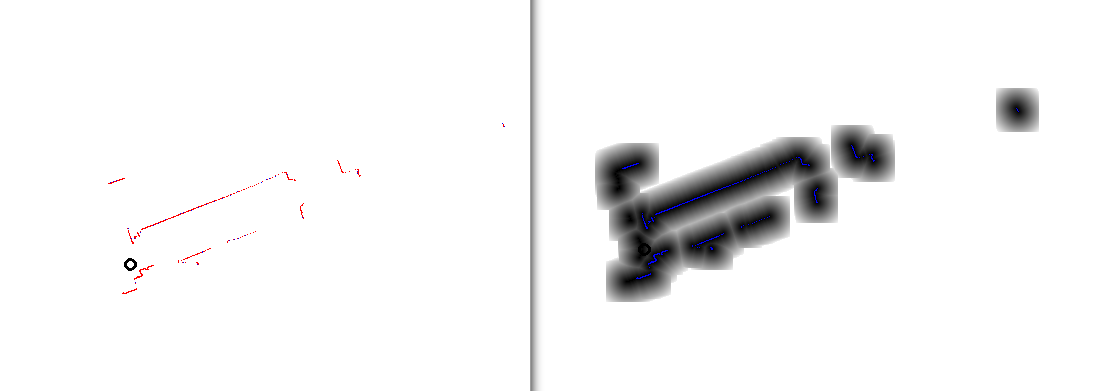
\includegraphics[width=0.8\textwidth]{resources/2d-lidar-mapping/ch6-scan-and-filed.png}  
	\caption{Real-time scan data and likelihood field data}  
	\label{fig:scan-and-field}  
\end{figure}

\subsection{Implementation of Likelihood Field Method (g2o)}
Below we demonstrate how to use the g2o optimizer \cite{Kummerle2011} to implement a likelihood field-based scan matching algorithm. By using an optimizer, we can more conveniently employ different iteration strategies and set robust kernel functions to achieve more robust matching algorithms. In fact, all the registration methods implemented earlier can be adapted to an optimizer-based approach. Now we define the $\mathrm{SE}(2)$ pose vertex and the observation error edges corresponding to each scan point.

\begin{lstlisting}[language=c++,caption=src/ch6/g2o\_types.h]
	class VertexSE2 : public g2o::BaseVertex<3, SE2> {
		public:
		EIGEN_MAKE_ALIGNED_OPERATOR_NEW
		
		void setToOriginImpl() override { _estimate = SE2(); }
		void oplusImpl(const double* update) override {
			_estimate.translation()[0] += update[0];
			_estimate.translation()[1] += update[1];
			_estimate.so2() = _estimate.so2() * SO2::exp(update[2]);
		}
	};
	
	class EdgeSE2LikelihoodFiled : public g2o::BaseUnaryEdge<1, double, VertexSE2> {
		public:
		EIGEN_MAKE_ALIGNED_OPERATOR_NEW;
		EdgeSE2LikelihoodFiled(const cv::Mat& field_image, double range, double angle, float resolution 
		= 10.0) : field_image_(field_image), range_(range), angle_(angle), resolution_(resolution) {}
		
		void computeError() override {
			VertexSE2* v = (VertexSE2*)_vertices[0];
			SE2 pose = v->estimate();
			Vec2d pw = pose * Vec2d(range_ * std::cos(angle_), range_ * std::sin(angle_));
			Vec2i pf = (pw * resolution_ + Vec2d(field_image_.rows / 2, field_image_.cols / 2)).cast<int>(); 
			
			if (pf[0] >= image_boarder_ && pf[0] < field_image_.cols - image_boarder_ && pf[1] >= 
			image_boarder_ && pf[1] < field_image_.rows - image_boarder_) {
				_error[0] = field_image_.at<float>(pf[1], pf[0]);
			} else {
				_error[0] = 0;
				setLevel(1);
			}
		}
		
		void linearizeOplus() override {
			VertexSE2* v = (VertexSE2*)_vertices[0];
			SE2 pose = v->estimate();
			float theta = pose.so2().log();
			Vec2d pw = pose * Vec2d(range_ * std::cos(angle_), range_ * std::sin(angle_));
			Vec2i pf = (pw * resolution_ + Vec2d(field_image_.rows / 2, field_image_.cols / 2)).cast<int>();
			
			if (pf[0] >= image_boarder_ && pf[0] < field_image_.cols - image_boarder_ && pf[1] >= 
			image_boarder_ && pf[1] < field_image_.rows - image_boarder_) {
				// Image gradient
				float dx = 0.5 * (field_image_.at<float>(pf[1], pf[0] + 1) - field_image_.at<float>(pf[1], pf[0] - 1));
				float dy = 0.5 * (field_image_.at<float>(pf[1] + 1, pf[0]) - field_image_.at<float>(pf[1] - 1, pf[0]));
				
				_jacobianOplusXi << resolution_ * dx, resolution_ * dy,
				-resolution_ * dx * range_ * std::sin(angle_ + theta) +
				resolution_ * dy * range_ * std::cos(angle_ + theta);
			} else {
				_jacobianOplusXi.setZero();
				setLevel(1);
			}
		}
		
		private:
		const cv::Mat& field_image_;
		double range_;
		double angle_;
		float resolution_ = 10.0;
		inline static const int image_boarder_ = 10;
	};
\end{lstlisting}

The Jacobian matrix here is consistent with our previous derivation, except that the likelihood field image has been moved inside the class for quick lookup of corresponding field function values and their gradients. Next, we only need to convert the iteration process from the Gauss-Newton method into an optimization problem.

\begin{lstlisting}[language=c++,caption=src/ch6/likelihood\_field.cc]
	bool LikelihoodField::AlignG2O(SE2& init_pose) {
		using BlockSolverType = g2o::BlockSolver<g2o::BlockSolverTraits<3, 1>>;
		using LinearSolverType = g2o::LinearSolverCholmod<BlockSolverType::PoseMatrixType>;
		auto* solver = new g2o::OptimizationAlgorithmLevenberg(
		g2o::make_unique<BlockSolverType>(g2o::make_unique<LinearSolverType>()));
		g2o::SparseOptimizer optimizer;
		optimizer.setAlgorithm(solver);
		
		auto* v = new VertexSE2();
		v->setId(0);
		v->setEstimate(init_pose);
		optimizer.addVertex(v);
		
		// Traverse source points
		for (size_t i = 0; i < source_->ranges.size(); ++i) {
			float r = source_->ranges[i];
			if (r < source_->range_min || r > source_->range_max) {
				continue;
			}
			
			float angle = source_->angle_min + i * source_->angle_increment;
			auto e = new EdgeSE2LikelihoodFiled(field_, r, angle, resolution_);
			e->setVertex(0, v);
			e->setInformation(Eigen::Matrix<double, 1, 1>::Identity());
			optimizer.addEdge(e);
		}
		
		optimizer.setVerbose(true);
		optimizer.initializeOptimization();
		optimizer.optimize(10);
		
		init_pose = v->estimate();
		return true;
	}
\end{lstlisting}

This implements the g2o-based 2D scan matching algorithm. By adding --method=g2o to the test program in Section~\ref{sec:likelihood-field}, you can test the optimizer version of likelihood field matching. Since the results are similar, we won't include result images in this section. Readers can also implement versions based on Ceres or other optimizers following similar principles. Additionally, we can perform linear interpolation on the likelihood field image (Figure~\ref{fig:scan-and-field}) to obtain more accurate error functions. We leave these two aspects as exercises.


